\documentclass[conference]{IEEEtran}
\usepackage[T1]{fontenc}
\usepackage[utf8x]{inputenc}
\usepackage[dvips]{graphicx}
\usepackage{latexsym}
\usepackage{subfig}
%\usepackage{float}
\usepackage{url}
%\usepackage{amsmath}

%\usepackage{ifpdf}
%\usepackage{cite}
\ifCLASSINFOpdf
  % \usepackage[pdftex]{graphicx}
  % declare the path(s) where your graphic files are
  % \graphicspath{{../pdf/}{../jpeg/}}
  % and their extensions so you won't have to specify these with
  % every instance of \includegraphics
  % \DeclareGraphicsExtensions{.pdf,.jpeg,.png}
\else
  % or other class option (dvipsone, dvipdf, if not using dvips). graphicx
  % will default to the driver specified in the system graphics.cfg if no
  % driver is specified.
  % \usepackage[dvips]{graphicx}
  % declare the path(s) where your graphic files are
  % \graphicspath{{../eps/}}
  % and their extensions so you won't have to specify these with
  % every instance of \includegraphics
  % \DeclareGraphicsExtensions{.eps}
\fi
\usepackage[cmex10]{amsmath}
%\usepackage{algorithmic}
%\usepackage{array}
%\usepackage{mdwmath}
%\usepackage{mdwtab}
%\usepackage{eqparbox}
%\usepackage[tight,footnotesize]{subfigure}
%\usepackage[caption=false]{caption}
%\usepackage[font=footnotesize]{subfig}
%\usepackage[caption=false,font=footnotesize]{subfig}
%\usepackage{fixltx2e}
%\usepackage{stfloats}
%\usepackage{url}
% correct bad hyphenation here
%\hyphenation{op-tical net-works semi-conduc-tor}

\begin{document}
\title{Relaxing CDN energy}

% author names and affiliations
% use a multiple column layout for up to three different
% affiliations


%\author{\IEEEauthorblockN{Michael Shell\IEEEauthorrefmark{1},
%Homer Simpson\IEEEauthorrefmark{2},
%James Kirk\IEEEauthorrefmark{3}, 
%Montgomery Scott\IEEEauthorrefmark{3} and
%Eldon Tyrell\IEEEauthorrefmark{4}}
%\IEEEauthorblockA{\IEEEauthorrefmark{1}School of Electrical and Computer Engineering\\
%Georgia Institute of Technology,
%Atlanta, Georgia 30332--0250\\ Email: see http://www.michaelshell.org/contact.html}
%\IEEEauthorblockA{\IEEEauthorrefmark{2}Twentieth Century Fox, Springfield, USA\\
%Email: homer@thesimpsons.com}
%\IEEEauthorblockA{\IEEEauthorrefmark{3}Starfleet Academy, San Francisco, California 96678-2391\\
%Telephone: (800) 555--1212, Fax: (888) 555--1212}
%\IEEEauthorblockA{\IEEEauthorrefmark{4}Tyrell Inc., 123 Replicant Street, Los Angeles, California 90210--4321}}


\author{\IEEEauthorblockN{Mohamad Dikshie Fauzie\IEEEauthorrefmark{1} \quad
Achmad Husni Thamrin\IEEEauthorrefmark{1} \quad
Rodney Van Meter\IEEEauthorrefmark{2} \quad
Jun Murai\IEEEauthorrefmark{2}}
\IEEEauthorblockA{\IEEEauthorrefmark{1}Graduate School of Media and Governance} \quad
\IEEEauthorblockA{\IEEEauthorrefmark{2}Faculty of Environment and Information Studies\\ 
Keio University, 252-0882 Kanagawa, Japan \\
dikshie@sfc.wide.ad.jp \quad\quad husni@ai3.net \quad\quad rdv@sfc.wide.ad.jp \quad\quad jun@wide.ad.jp}
}
% make the title area
\maketitle
\IEEEpeerreviewmaketitle

\begin{abstract}

Many CDN companies utilize peer-to-peer to scaling the services and saving bandwidth.
However, we still have little knowledge about the energy consumption in peer-assisted CDN.
This paper presents an analysis of a energy consumption in peer-assisted CDN system, where an ISP manages its own CDN and its users participate in a P2P network to assist content delivery.
To evaluate energy consumption in peer-assisted CDN, we take two cases: (1) live stream and (2) online storage.
We developed a simple energy consumption model for live streaming service and online storage service and evaluate this model using a empirical existing live streaming model and online storage model.
We find that in live streaming service, total energy system increase with growing number of peers.
However, if we concern only on CDN service part, delegate part of workload to peers can save CDN server up to $11\%$ compare to pure CDN architecture, while total energy system difference with pure CDN only less than $1\%$. 
In peer assisted online storage, we study three server bandwidth allocation strategies: (1) theoretical lower bound, (2) request driven, and (3) water level.  
total energy system depends on strategies of server bandwidth allocation.
Compare to pure CDN architecture peer-assisted, peer assisted online storage total system energy saving less than $1\%$.
\end{abstract}


%\begin{keyword}
%CDN, Data Center, Energy, Peer Assisted, P2P
%\end{keyword}

\maketitle

%1
\section{Introduction}\label{intro}
Streaming content, especially video, represents a significant fraction of the traffic volume on the Internet, and it has become a standard practice to deliver this type of content using Content Delivery Networks (CDNs) such as Akamai and Limelight for better scaling and quality of experience for the end users.  
For example, Youtube uses Google cache and MTV uses Akamai in their operations.

With the spread of broadband Internet access at a reasonable flat monthly rate, users are connected to the Internet 24 hours a day and they can download and share multimedia content.  
P2P (peer to peer) applications are also widely deployed.  
In China, P2P is very popular; we see many P2P applications from China such as PPLive, PPStream, UUSe, Xunlei, etc.  
Some news broadcasters also rely on P2P technology to deliver popular live events.  
For example, CNN uses the Octoshape solution that enables their broadcast to scale and offer good video quality as the number of users increases.

From the Internet provider point of view, the presence of so many always-on users suggests that it is possible to delegate a portion of computing, storage and networking tasks to the users, thus creating P2P networks where users can share files and multimedia content.
Starting from file sharing protocols, P2P architectures have evolved toward video on demand and support for live events.

Broadband network access helps P2P applications to perform better.
xDSL networks are deployed worldwide, and in some countries, such as Japan, even higher bandwidth fiber to the home (FTTH) already exceeds DSL in market penetration.  In the coming years, FTTH will be massively deployed by network operators throughout the world.  
As access bandwidth increases, P2P systems may become more efficient since a peer can contribute much more.

In Peer assisted CDN \footnote{in this paper, we may interchange Peer Assisted CDN and CDN-P2P.}, users can download content from CDN nodes for from other users or peers the content.
A user may cache the content after download to serve requests from other users
Due to complexity of behavior of peers, the process should be done in home gateway user where ISP can have control on it. 

On the other hand, data center where CDN server placed faces costs for powering the data center.
The Uptime Institute, a global data center authority, surveyed 1100 data center owners and operators on 2012, reported that 55\% organizations must increase budget 10\% than 2011 \cite{uptime}.  
30\% of organizations will run out of data center capacity (power, cooling, space, and network) in the end of 2012 \cite{uptime}. 
More than 50\% organizations surveyed reported that saving energy \footnote{in this paper, we may interchange energy and power.} is major priority \cite{uptime}.
Even in the data centers using the state of art cooling technologies heat dissipation accounts for at least $20\%$ until $50\%$ of the total power consumption 
\cite{google}.
The increases in energy cost and the demand due to growth of traffic urges the data center operators and owners to look for ways to reduce energy usage in the years to come.
Although reducing energy consumption can effectively reduce overall cost, this will limit the capacity growth and scalability of the service provisioning.
For example: routers and servers spend most of their energy on the baseline activities such as running the fans, spinning hardisks, powering backplane, and powering the memory. 
Even in an idle state, modern systems can be consuming anything from $50\%$ until $80\%$ of the power consumed under maximum load \cite{4404806,4509688}.
Alternatively, the data center and be revamped by relocating some services to end-host computers or peers.
Peers contribute their communication, storage, and computation resources to exchange data and provide services while the data center performs central administration and authentication as well as backend processing.
P2P network, formed by peers offer flexibility and scalability in service delivery.
%Therefore, P2P services can assist and enhance data center.
It is not our aim to advocate one system architecture over another.
Many issue such as manageability, reliability, and ease of deployment must be taken into account when making high level architectural decisions.

In this paper, we study the energy consumption of hybrid CDN-P2P.  
It has been known that CDN energy consumption is better than P2P architecture \cite{feldmann2010energy,baliga2007energy}, unfortunately that model only think small part of problem energy consumption (devices/hardwares).
To be fair, we also need to see how combination of some architectures can help to reduce energy footprint, for example: combination of CDN and P2P.
%If we can move part of computation resource from CDN in data center to P2P, then we can relax power budget of data center for hardware and cooling. 

The rest of this paper is organized as follows. 
Section 2 present motivation of this paper.
Section 3 provides an overview of system model and energy model.  
In section 4, we will present result and analysis.  
Section 5 will conclude this paper. 

\section{Motivation}\label{motivation}
CDN architectures are host-oriented: content is delivered to end users through host servers that are centrally managed in a few data centers.
The growing of Internet traffic dominated by video, the energy consumption of a host oriented architecture becomes problematic due to over provisioning factor.
The idea of utilizing the user's computation power to support ISP operation is not new. 
The figaro project proposed residential gateway as an integrator of different networks and services, becoming an Internet wide distributed content management for a proposed future Internet architecture.  
The important key in this architecture is both user home gateway and access bandwidth controlled and managed by ISP.
In this case, ISP can offload part of workload on their CDN to user's home gateway.  
By offloading workload, their CDN can relax energy demand thus relaxing data center power budget or relaxing capacity planning for power.
This architecture depends largely on the number of devices which can be found online at a point in time.
While some users keep their home gateway online at all times, there are small number of users might turn off or their home gateway can not be reached.
Based on study from Dischinger et al., \cite{Dischinger:2007:CRB:1298306.1298313} and Valancius et al., \cite{valancius2009greening}, the average availability of the residential gateways in 12 major ISPs over one month is up $85\%$ with $5\%$ until $8\%$ uptime variations thought out a day thus residential gateway has potential to use as peers.

\section{System Description}\label{system model}
\subsection{Live Streaming}

\begin{figure}[thb]
\begin{center}
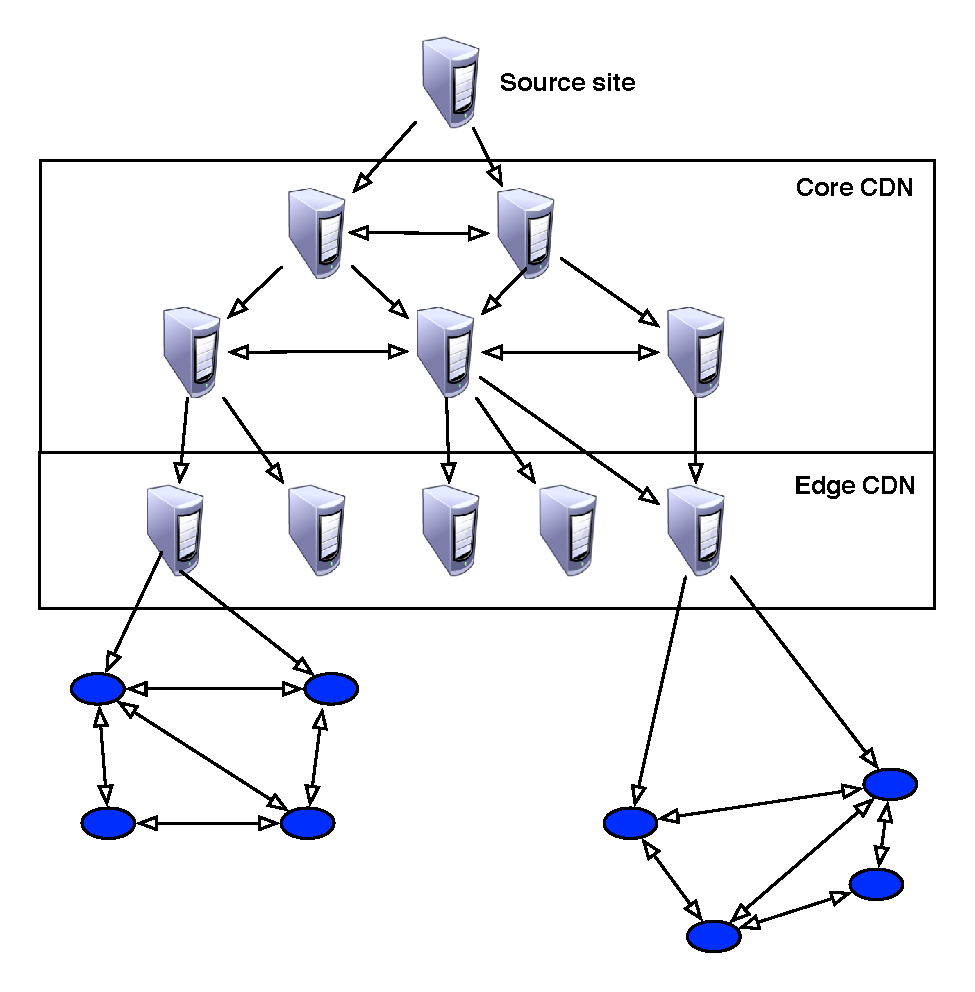
\includegraphics[scale=0.4]{graphs/livesky.eps}
\end{center}
\caption{Example model of live stream content delivery architecture with peer assisted.}
\label{fig:iptv}
\end{figure} 

Figure \ref{fig:iptv} shows example model of CDN with peer assisted for live streaming adapted from \cite{Yin:2010:LEC:1823746.1823750}.
CDN server deliver video contents from content providers to end users. 
The CDNs are organized into severaltiers according to the scale demand, meanwhile satisfying the QoS and reliability requirement. 
Edge CDNs are directly responsible for serving end users and the remaining part are core CDN.
The goal of the server side overlay is efficient data distribution with some measures to guard against some node failures and network delay.
Since CDNs are more stable, the server side distribution overlay is largely tree-based. 
However, to provide greater reliability in the presence of node or network failures, CDN is allowed to retrieve the content either from CDN higher up in the hierarchy or from peer CDN in the same level.
Edge CDNs are responsible for serving end users, they are typically heavily loaded. 
In this system, a peer that is served by edge CDN named as seeders while a peer that is served by seeders named as leechers. 

Before accessing the video stream, a peer first obtain the URL from content source.  
The global load server balance takes into account the peer location, edge CDN location, and edge CDN load to find a suitable edge CDN for this peer.
The peer is then redirected to this edge CDN.
The edge CDNs are preconfigured with some decision logic that decides if a new peer should be served directly by edge CDN or it should be redirected to P2P overlay.

In P2P transmission overlay, the stream is seperated into several substreams according the stream id.
For example, if the video is divided into six substreams, substream-0 consists of frames $0,6,12,18,...$ , substream-1 consists of frames $1,7,13,19,..$ and so on. 
Peers are organized in a tree-based overlay on a per-substream basis.
Each peer has a parent node for each substream and obtain the stream frames belonging to this substream from the parent node. 
Additionally, in order to be robust to network or node failures, peers also construct a mesh-style overlay to retrieve missing frames for continuous playback.
The working environment for peer-assisted CDN live streaming system is defined by several parameters such as: (1) media playback bitrate, (2) the total number of end users, (3) the bandwidth capacity of the edge CDNs, and (5) Characteristics of end users such as their upload bandwidth capacity and churn rates. 
Given the working environment, the control parameter is the number of end users that are served directly by the edge CDNs.
Maximum number of seeders is bounded by maximum CDN's capacity, while maximum number of leechers are bounded by number of seeders can support the bitrate.
Denote number of seeders is $n_s$, number of leechers is $n_l$, $\rho$ is maximum bitrate that supplied by seeders to leechers, and $r=1$ is video bitrate, therefore we have number of leechers that can be supported by seeders is:

\begin{equation}\label{eqn:leecher}
	\lfloor n_l \rfloor = n_s . \rho
\end{equation}

Number of seeders that support or upload content to leecher is:

\begin{equation}\label{eqn:seeders-to-leechers}
	n_{s}^{u} = n_l . \frac{r}{\rho}
\end{equation}

The illustration as follows, suppose we have video bitrate $r=1$, seeder upload rate $\rho=0.25$, and maximum CDN capacity is $643Mbps$. 
Maximum number of seeders supported by CDN is $n_s=643$.
Maximum number leechers supported by seeders is $n_l=160$.  
Number of seeders that upload content to leechers is $n_{s}^{u}=640$.  
Therefore we have three seeders that do not need to upload content to leecher. 

\subsection{Peer Assisted Online Storage}

\begin{figure}[thb]
\begin{center}
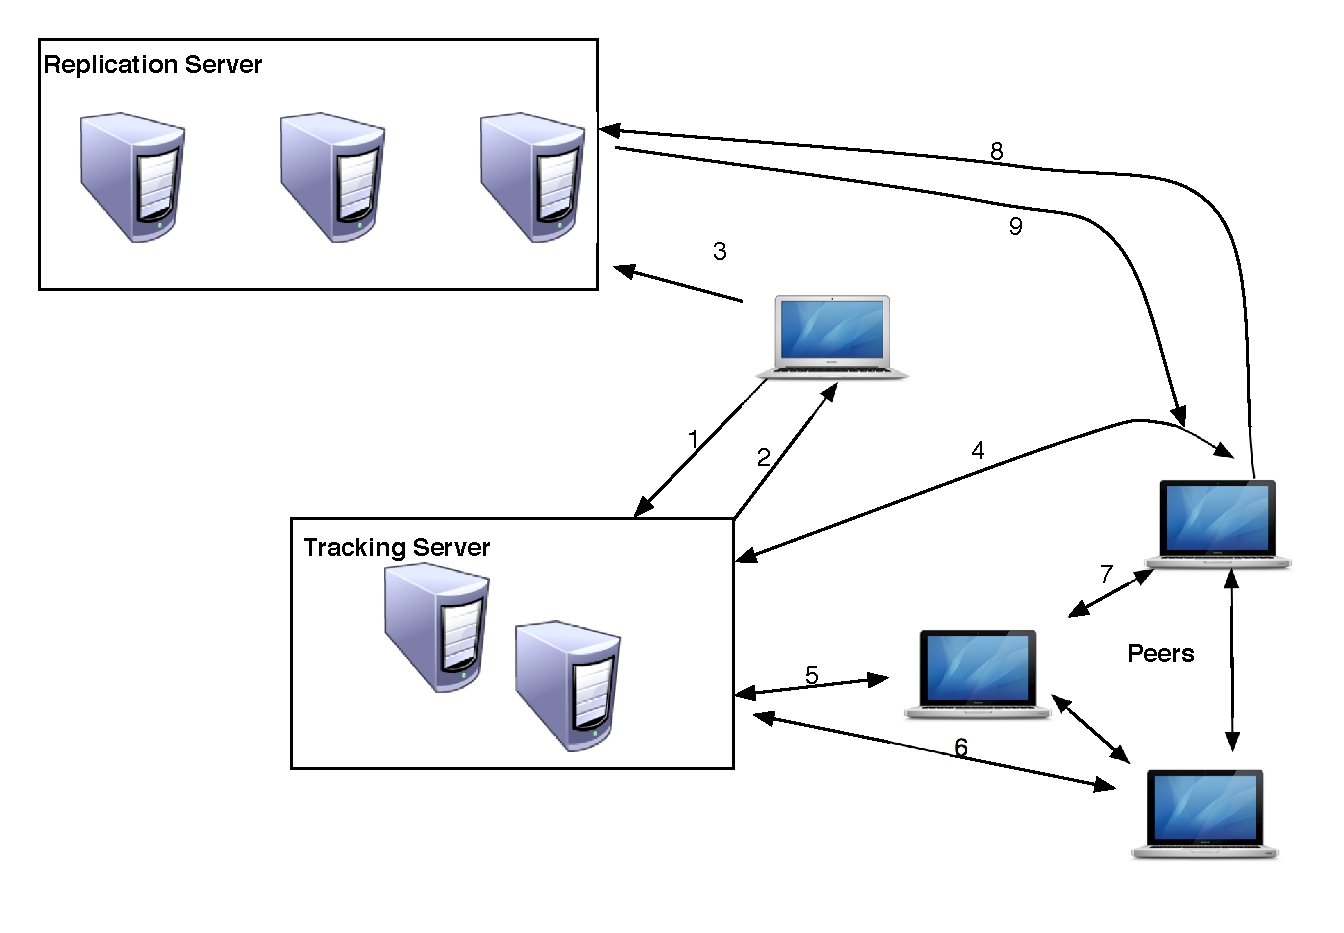
\includegraphics[scale=0.4]{graphs/fs2you-arch.eps}
\end{center}
\caption{Example model of peer-assisted online storage architecture.}
\label{fig:fs2you}
\end{figure} 

Figure \ref{fig:fs2you} illustrates the architecture of peer-assisted online storage for file hosting system (one-click hosting services with peer-assistance) \cite{5061997}.
Each file provided by users is treated as a swarm, since it is distributed live on an ongoing basis to other users. 
Each end user is treated as a peer, inheriting the terminology of pure P2P systems.
In fig.\ref{fig:fs2you} arrows 1,2,and 3 represent the interaction between a participating peer and dedicated tracking and replication servers for uploading new content.
Arrows 4,5, and 6 represent the interaction between peers and the tracking server to maintain the peer topology. 
Arrow 7 represents the sharing of file blocks and exchange of availability among peers. 
Arrows 8 and 9 represent peer requests and server response when the requests cannot be satisfied by other peers alone. 

Tracking server serves the purpose of maintaining swarm information and bootstrapping peers.
Specifically, it maintains a unique swarm ID and a secure hash value for each file provided by a peer and keeps track of the group of users that are participating in the distribution of each swarm. 
Replication servers serve as dedicated content servers to maintain availability of swarms when they are not actively served by peers alone. 
All peers involved in the system, i.e., either downloading the file in the system of holding a replica of the file, are organized into a topology, so that block availability information can be exchanged and blocks can be shared among neighboring peers in the topology.
When a downloading peer join the swarm, it contacts the tracking server and obtains a list of initial partners (determined by a system) that are randomly selected from peers associated with the same channel.  
This partnership list is periodically updated and new partners can be added. 
Partners can be active or inactive, which is determined by whether there are actual connections and data block transfer between the peer and its partners.

Peers need to keep a reasonably number of active and inactive partners in order to maintain a sustainable level of downloading efficiency and to be resilient to network dynamics. 
Each peer can have up to $N$ partners in its pool of inactive partners, which is related to the number of peers simultaneously being online in a swarm.
In case the size of the inactive partner pool increases to over threshold $N$, a peer will discard aged partners or partners who it has failed to establish a connection with. 
On the other side, with respect to active partners, the maximum number per swarm that peer can have is bounded by a system parameter $K_{max}$.
Connections to active partners can be broken from time to time due to various reasons, such as slow downloading rates and idling for a long time.
Each peer periodically monitors the number of its current partner. 
If the number of active partners falls below a threshold $K_{min}$ , it exchanges active partner lists with its current active partners through gossip and attempts to establish new connections with a random subset of inactive partners.
If successful, the status of these inactive partners will be promoted to active. 

To maintain accurate list of peers in each swarm, peers report their status to the tracking server periodically which contains vital peer information such as unique peer identifier, its IP address, and information about swarms that it has joined. 
Since each peer can be potentially involved in a large number of swarms, to keep overhead low, the reported status only includes information of a bounded number of top $C$ swarms, including swarm identifier and download ratios, defined as the amount of file that has been downloaded so far. 
The top $C$ swarms represent files that have been downloaded by this peer, ranked by a value computed by the combination of the file size, download ratio, and the time when the peer joined the swarm. 
Upon receiving status reports from peers, the tracking server periodically updates the corresponding list of peers associated with each swarm.
Such a periodic refresh of peer lists in each swarm (associated to each file) assists peers to gain access to active partners that are most helpful, with a reasonable level of overhead. 
Consequently, the downloading performance can be improved and the load on servers can be alleviated. 

In content distribution strategies, each file is divided into fixed size blocks.
A block map (BM) is introduced to specify the availability of blocks at each peer. 
The periodic exchange of BMs among peers enable them to locate the needed blocks. 
Each peer can retrieve a number of distinct blocks from multiple active partners simultaneously up to the number of its current active partners.
If multiple partners hold a desired block, a peer will randomly choose one of its active partners to request that block.
Since server hold important role in this system, we present simple mathematical model of server bandwidth allocation strategies \cite{4024139,Sun:2009:POS:1542245.1542249} as base for energy calculation later in Sec.\ref{subsec:onlinestorage} as follows:\\
type-1 represents less popular files and type-2 represents popular files. \\
$S_{t1}$ represents server bandwidth allocated to a file type-1 and $S_{t2}$ represents server bandwidth allocated to a file type-2. \\
$S$ is total server bandwidth. \\
$S_{max1}$ is the maximum amount of server bandwidth that can be assigned to a file of type-1 and $S_{max2}$ is the maximum amount of server bandwidth that can be assigned to a file of type-2.\\
$M_{t1}$ is number of type-1 files and  $M_{t2}$ is number of type-2 files.\\
$\lambda_{t1}$ is the arrival rate of new peers in type-1 file and $\lambda_{t2}$ is the arrival rate of new peers in type-2 file.\\
$\lambda = M_{t1}.\lambda_{t1} + M_{t2}.\lambda_{t2}$\\
$M=M_{t1} + M_{t2}$.\\
$\eta$ is the file sharing effectiveness. It is the fraction of the upload capacity of peers that is being utilized.\\

There are three server bandwidth allocation strategies:  (1) lower bound of the average downloading time; (2) request driven strategy; (3) water leveling strategy.
In lower bound of the average downloading time, we shall first assign the server bandwidth to type-1 files until $S_{t1}$ reaches its maximum value then the residual server bandwidth can be assigned to type-2 files.
This strategy to achieve the lower bound of the system wide average downloading time is also applicable to the general case of multiple types of files: the server should always satisfy the requests from the peers who are downloading the least popular files.\\
In request driven strategy, the server serves every request from peers. 
The server bandwidth is equally divided among all the peers.
We assume that the number of requests for a file to the server is proportional to the peer arrival rate of the file. 
We also assume that when the amount of server bandwidth assigned to one of the two types of files has reached its maximum value, the residual server bandwidth will be assigned to the other type of files.\\
In water leveling strategy, this strategy equalizes the server bandwidth across all the files by taking file popularity into consideration. 
The server serves the requests from peers according to a certain probability which is inversely proportional to the peer arrival rate of the file.
We assume that the number of requests for a file to the server is proportional to the peer arrival rate of the file, the server will serve the same number of requests for different files and therefore the server bandwidth is equally allocated across all the files.\\
Average downloading time can be calculated as \cite{Sun:2009:POS:1542245.1542249}:
\begin{equation}\label{eqn:averagetimedownload}
\begin{split}
T_d &= \frac{1}{M_{t1}.\lambda_{t1} + M_{t2}.\lambda_{t2}}(\frac{M_{t1}.f_{t1}.\lambda_{t1}.\eta_{t2} + M_{t2}.f_{t2}.\lambda_{t2}.\eta_{t1}}{\mu.\eta_{t1}.\eta_{t2}}  \\ 
   & - \frac{S_{t1} (M_{t1}.\eta_{t2}-M_{t2}.\eta_{t1}) + S.M_{t2}.\eta_{t1}}{\mu.\eta_{t1}.\eta_{t2}}) 
\end{split}	
\end{equation} 
next, we can calculate number of peers as \cite{Sun:2009:POS:1542245.1542249}:
\begin{equation}\label{eqn:numofpeers}
\begin{split}
\sum x_i = T_d . \sum \lambda_i
\end{split}	
\end{equation} 


\subsection{Energy Model}\label{energy model}
In this paper, our goal is to provide a general view and a fair comparison of the energy consume by a CDN and hybrid CDN-P2P architecture. 
To do so, we designed a series of model and perform an analysis.
Our energy model is similar to the models used in \cite{Nedevschi:2008:HDC:1855610.1855618}.
The difference with \cite{Nedevschi:2008:HDC:1855610.1855618}, firstly, our baseline energy is not function of bitrate flow. 
Our baseline energy is based on minimum energy required to turn-on the device without any traffic low trough the device. 
Secondly, our overhead number based on COP value.

For each component, we consider two energy measurement:  baseline energy consumption and energy consumed per work unit $\delta$.
The baseline energy is the energy consumed to keep the device on.
Even when there is no traffic, the device still consume energy.
The energy consumption for a single request in CDN server as:
\begin{equation}\label{eqn:E_d}
	E_{d} = E_s
\end{equation}
while the energy consumption for a single request in network as:
\begin{equation}\label{eqn:E_r}
	E_{r} = d_s.E_r
\end{equation}
and energy of peer or client is $E_p$.

where $d_s$ is number of hops or the path length.
We define $\delta_s$ and $\delta_r$ work-induced energy consumed per additional bit transferred by a server and router.   
We can express these per-bit work induced consumptions as follows:
\begin{equation}\label{eqn:delta_s}
	\delta_s = \frac{(S_{max} - S_{base})}{M_s} 
\end{equation}
$S_{base}$ is a server's baseline power consumption.  
$S_{max}$ is a server's power when operating at maximum capacity.
$M_s$ is the maximum capacity in bit per second for a server.
Same formulation also applied for network component.  
\begin{equation}\label{eqn:delta_r}
	\delta_r = \frac{(R_{max} - R_{base})}{M_R} 
\end{equation}
$R_{max}$ is a router power when operating at maximum capacity.
$R_{base}$ is a router's baseline power consumption.
$M_R$ is maximum capacity in bit per second for a router.

Substituting eq.\ref{eqn:delta_s}, and eq.\ref{eqn:delta_r} to eq.\ref{eqn:E_d} and eq.\ref{eqn:E_r}, we can rewrite eq.\ref{eqn:E_d} and eq.\ref{eqn:E_r} as follows:
\begin{equation}\label{eqn:E_d dan E_r}
\begin{split}
	E_{d} &= \delta_s.B + E_{s-baseline}\\
	E_{r} &= d_s.\delta_r.B + E_{r-baseline}\\
	E_{p} &= \delta.B + E_{p-baseline}
\end{split}
\end{equation}
Finaly total energy is:
\begin{equation}\label{eqn:E_t}
\begin{split}
	E_{t} &= E_d + E_r + E_p \\
	E_{t} &= \delta_s.B + E_{s-baseline} + d_s.\delta_r.B \\
	      &+ E_{r-baseline} + \delta_p.B + E_{p-baseline}
\end{split}
\end{equation}
where $B$ is size of file to be transferred. 

We have shown energy model for server, router, and peer.  
Now, we introduce the overhead for server and router. 
Overhead that we will consider here is cooling power.  
Since servers and routers are placed in data center, data center seek to provision the cooling adequately to extract the heat produce by servers, switches, routers, and other devices.
Practically, cooling provisioning are done at facilities level.
Data center operator operate cooling facilities based on power ratings of servers, switches, routers, and other devices often with some additional headroom for risk tolerance. 

The cooling cycle of a typical data center operates in the following way:
Cooling units operate by extracting heat from the data center and pumping cold air into the room, usually through a pressurized floor plenum.
The pressure forces the cold air upward through vented tiles, entering the room in front the hardware
Fans draw the cold air inward and through the server; hot air exits through the rear of the server.
The hot air rises sometimes with the aid of fans and a ceiling plenum , and is sucked back to the cooling units.
The cooling units force the hot air past pipes containing cold air or water. 
The heat from the returning air transfer through the pipes to the cold substance. 
The heated substance leaves the room and goes to a chiller and cooling unit fans force the cold air back into the floor plenum. 
%Above process is shown in fig.\ref{fig:datacenter}

The efficiency of this cycle depends on several factors, including the conductive substance and the air flow velocity, but it is quantified by coefficient of performance (COP).
The COP is the ratio of heat removed ($Q$) to the amount of work necessary ($W$) to remove that heat  \cite{moore2005making}:

\begin{equation}\label{eqn:cop}
	COP=\frac{Q}{W}
\end{equation}

Therefore, the work necessary to remove heat is inversely proportional to the COP.  
A higher COP indicates a more efficient process, requiring less work to remove a constant amount of heat.

However, the COP for a cooling cycling is not constant, increasing with the temperature of the air the cooling unit pushes into the plenum.  
COP value empirically can be computed using \cite{moore2005making}:
\begin{equation}\label{eqn:copt}
	COP(T) = 0.0068.T^2 + 0.0008.T + 0.458
\end{equation}
Where $T$ is temperature supply by cooling unit.  

\begin{figure}[thp!]
\begin{center}
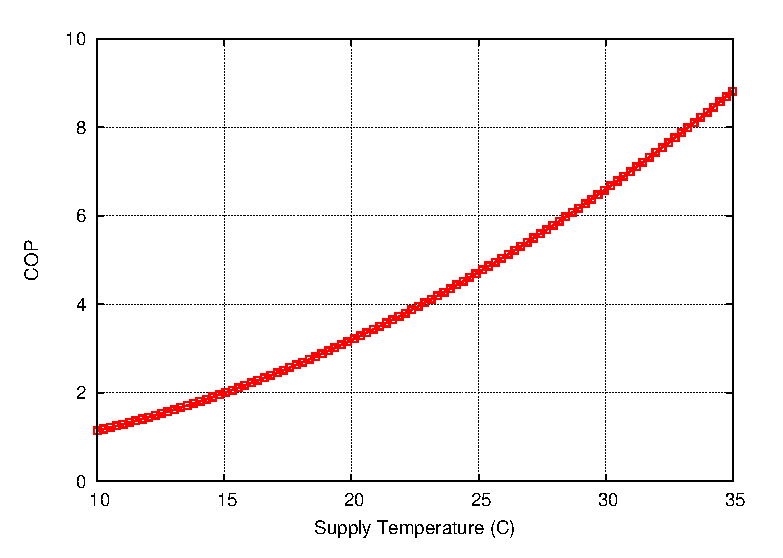
\includegraphics[scale=0.6]{graphs/cop.eps}
\end{center}
\caption{COP curve for the chilled water cooling units from HP Lab utility data center.
As the target temperature of the air the cooling unit pumps into the floor plenum increases, the COP increases \cite{moore2005making}.}
\label{fig:twotier}
\end{figure} 

Cooling cost can be calculated as  \cite{moore2005making} :

\begin{equation}\label{eqn:cost}
C = \frac{Q}{COP(T)}
\end{equation}

Where $Q$ is amount of power the servers and hardwares consume.
Currently we assume a uniform $T$ from each cooling units due to the complications introduced by non-uniform cold air supply.

Considering cooling energy overhead, we can substitute eq.\ref{eqn:cost} to eq.\ref{eqn:E_t}, therefore total energy consumption: 
\begin{equation}
	\hat{E}_{t} = E_{d}.\left( 1+\frac{1}{COP(T)} \right) + E_{r}.\left( 1+\frac{1}{COP(T)} \right) + E_p
\end{equation}

We do not include cooling overhead in peer energy consumption because most of peers in home do not need cooling.  
The air conditioning in home mainly for human not for devices.

\section{Result and Discussion}\label{analysis}

\begin{table}[htp!]
\caption{Numerical Simulation Parameters from \cite{Nedevschi:2008:HDC:1855610.1855618}, \cite{valancius2009greening},\cite{4509688}, and \cite{Sun:2009:POS:1542245.1542249}.}
\label{tab:simparameters}
\hbox to\hsize{\hfil
\begin{tabular}{l|l}\hline\hline
Symbol & Value\\\hline
$\delta_s$ & $5.2 . 10^{-8}$ (J/b)\\
$\delta_r$ & $8.0 . 10^{-9}$ (J/b)\\
$\delta_p$ & $16 . 10^{-9}$ (J/b)\\
$E_{r-baseline}$ & $750$ watt \\
$E_{s-baseline}$ & $290$ watt \\
$E_{p-baseline}$ & $13.5$ watt \\
$d_s$ & $1$ \\
$N_{s}^{u}$ & $[0.25,0.5,0.75,1]$ Mbps \\
$N$ & $[100,..,1000]$ \\
$\lambda_{t1}$ & $0.1$\\
$\lambda_{t2}$ & $1$\\
$\eta_{t1}$ & $0.5$ \\
$\eta_{t2}$ & $1$ \\
$M_{t1}$ & $10$ \\
$M_{t2}$ & $1$ \\
$f_{t1} = f_{t2}$ & $100$ MB\\
$\mu$ & $0.5$ Mbps\\
$c$ & $1$Mbps\\
$T$ & $[20,25]$ correspond to COP value $[3.194,4.728]$\\\hline
\end{tabular}\hfil}
\end{table}

\begin{figure}[htp!]
\begin{center}
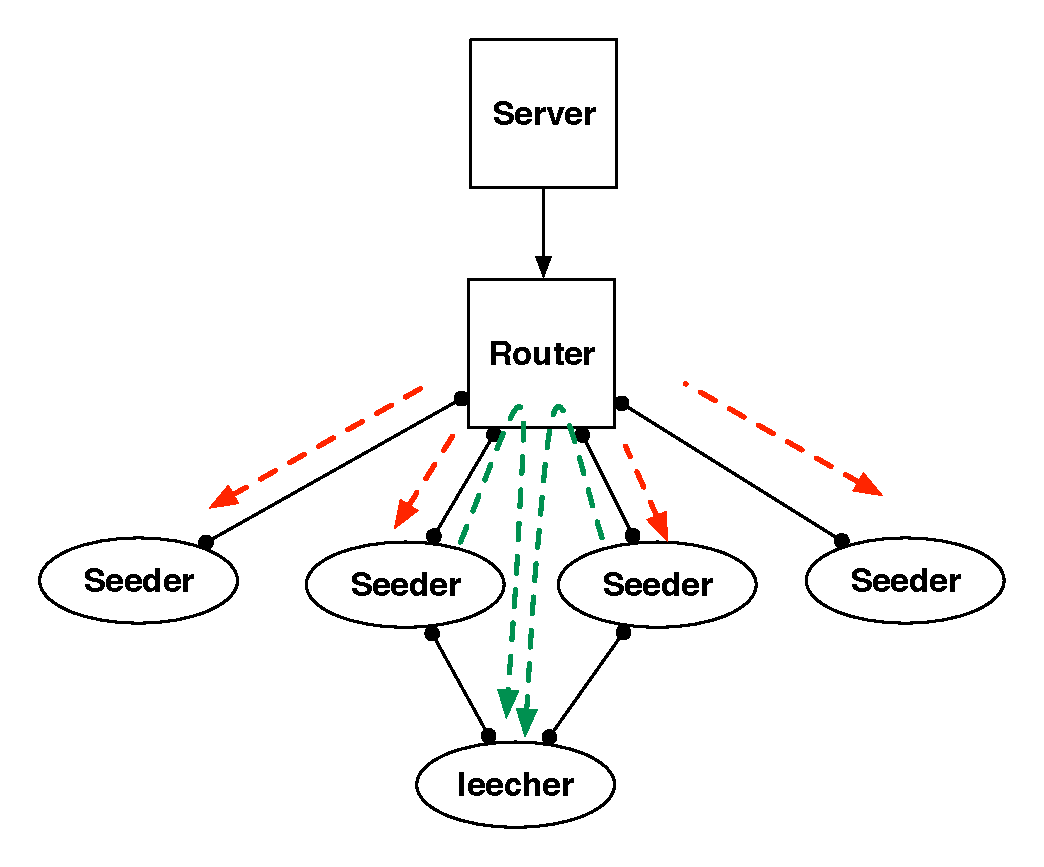
\includegraphics[scale=0.35]{graphs/topology.eps}
\end{center}
\caption{Physical representation of the network.}
\label{fig:dummy}
\vspace{-2mm}
\end{figure} 


\begin{figure*}[htp!]
\centering
\begin{minipage}[b]{0.4\linewidth}
	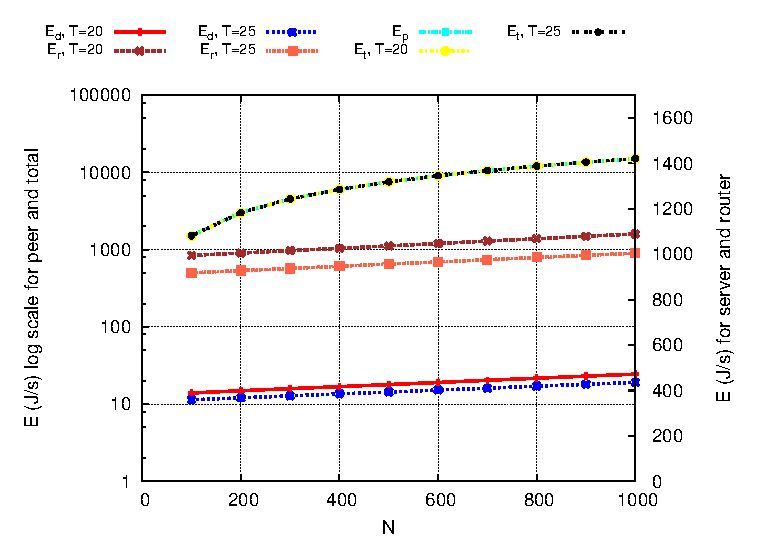
\includegraphics[scale=0.6]{graphs/cdn.eps}
	\caption{Power consumption in CDN architecture.}
	\label{fig:4-0}
\end{minipage}
\hfill
%\begin{minipage}[b]{0.4\linewidth}
%	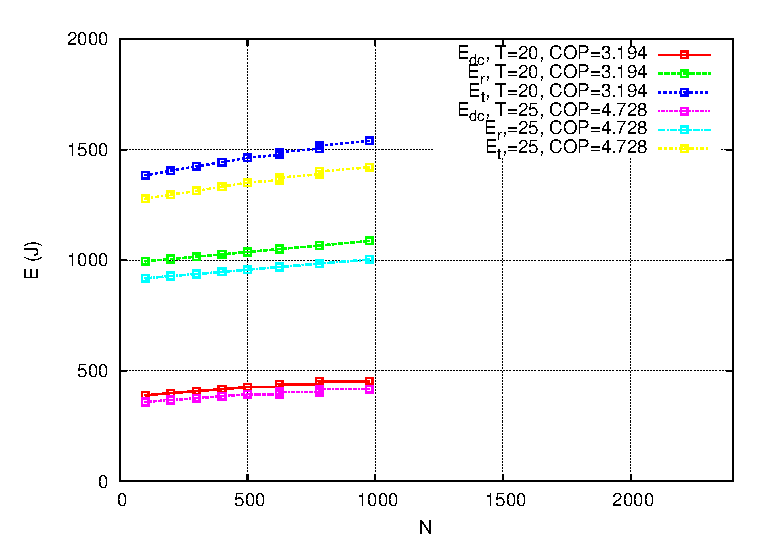
\includegraphics[scale=0.5]{graphs/cdnp2p-1.eps}
%	\caption{CDN-P2P $\rho=0.25$.}
%	\label{fig:4-1}
%\end{minipage}
%\hfill
%\begin{minipage}[b]{0.4\linewidth}
%	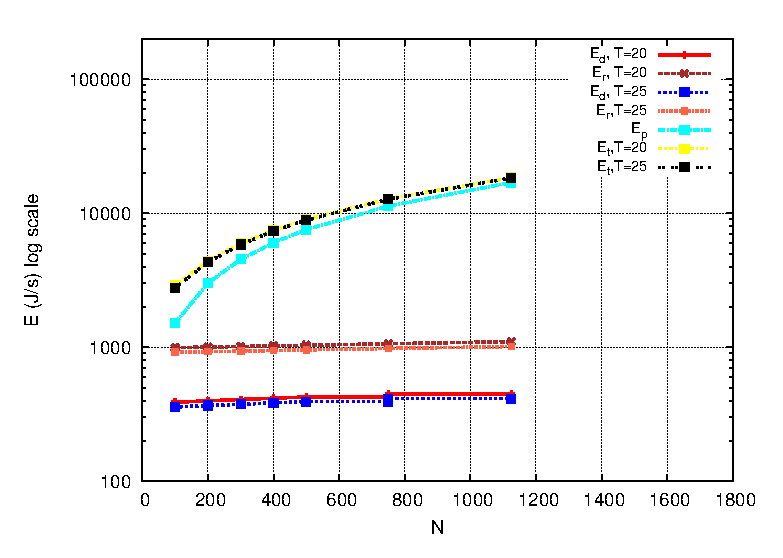
\includegraphics[scale=0.5]{graphs/cdnp2p-2.eps}
%	\caption{CDN-P2P $\rho=0.5$.}
%	\label{fig:4-2}
%\end{minipage}
%\hfill
\begin{minipage}[b]{0.4\linewidth}
	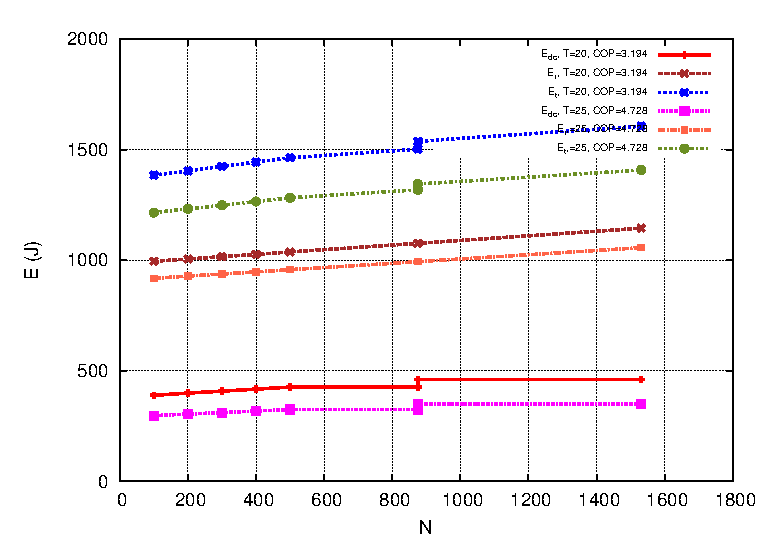
\includegraphics[scale=0.6]{graphs/cdnp2p-3.eps}
	\caption{Power consumption in CDN-P2P architecture with $\rho=0.75$.}
	\label{fig:4-3}
\end{minipage}
%\hfill
%\begin{minipage}[b]{0.4\linewidth}
%	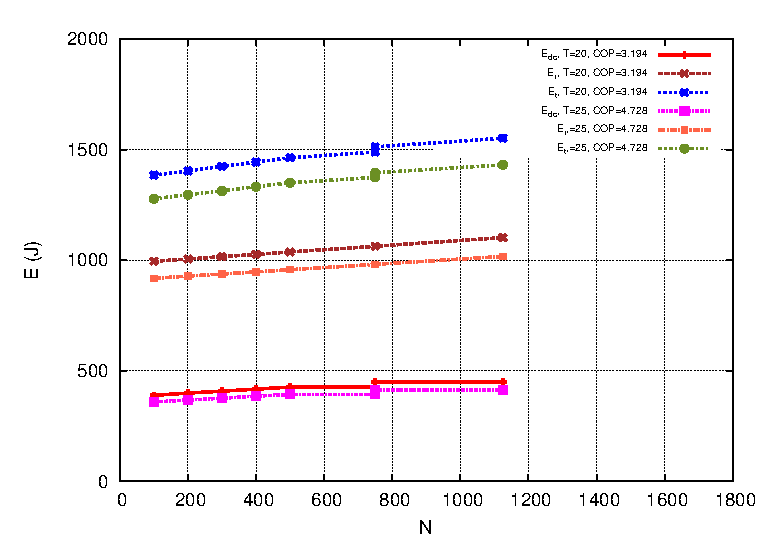
\includegraphics[scale=0.5]{graphs/cdnp2p-4.eps}
%	\caption{CDN-P2P $\rho=1$.}
%	\label{fig:4-4}
%\end{minipage}
\label{fig:main}
\end{figure*}

\begin{figure*}[htp!]
\centering
\begin{minipage}[b]{0.4\linewidth}
	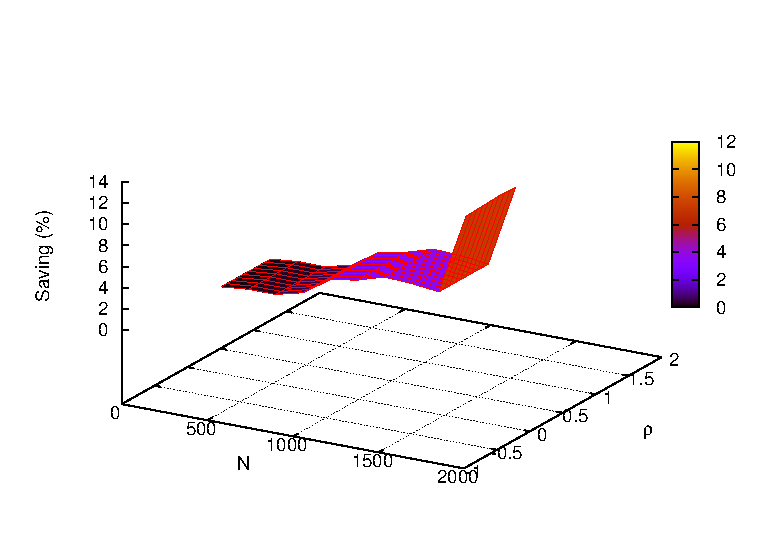
\includegraphics[scale=0.5]{graphs/diff3dimension.eps}
	\caption{Different power consumption between CDN and CDN-P2P for CDN server component with $\rho=0.25,0.5,0.75,1$.}
	\label{fig:diff1}
\end{minipage}
\hfill
\begin{minipage}[b]{0.4\linewidth}
	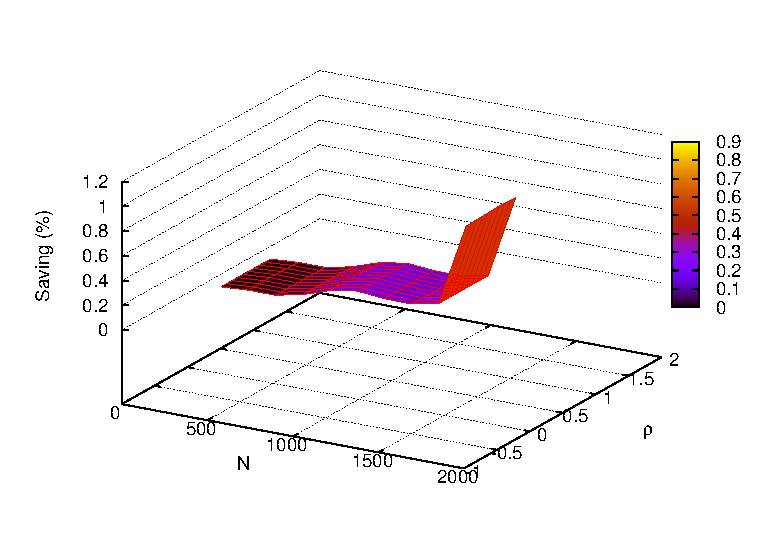
\includegraphics[scale=0.5]{graphs/diff3dimension2.eps}
	\caption{Different power consumption between CDN and CDN-P2P for total system with $\rho=0.25,0.5,0.75,1$.}
	\label{fig:diff2}
\end{minipage}
\label{fig:maindiff}
\end{figure*}

\begin{figure*}[htp!]
\centering
\begin{minipage}[b]{0.4\linewidth}
	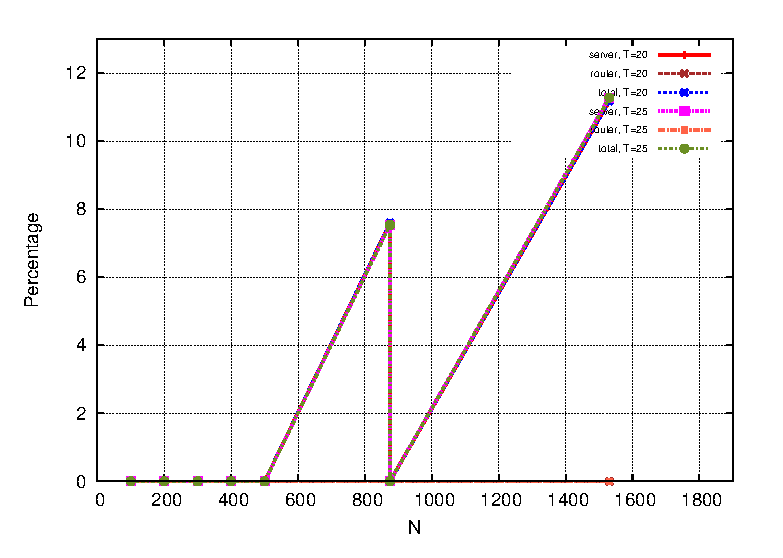
\includegraphics[scale=0.5]{graphs/diff-3.eps}
	\caption{Different power consumption between CDN and CDN-P2P for CDN server component with $\rho=0.75$.}
	\label{fig:diffs1}
\end{minipage}
\hfill
\begin{minipage}[b]{0.4\linewidth}
	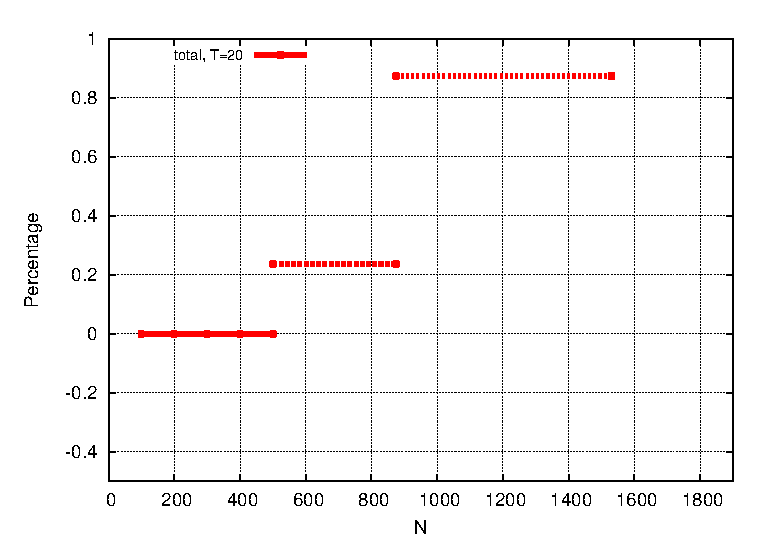
\includegraphics[scale=0.5]{graphs/diff-3-total.eps}
	\caption{Different power consumption between CDN and CDN-P2P for total system with $\rho=0.75$.}
	\label{fig:diffs2}
\end{minipage}
\label{fig:maindiff2}
\end{figure*}



\subsection{Numerical Parameters}\label{sec:parameters}
The parameters used in this numerical simulation were adapted from \cite{Nedevschi:2008:HDC:1855610.1855618}, \cite{valancius2009greening}, \cite{4509688} and \cite{Sun:2009:POS:1542245.1542249}. 
Parameters values is shown in table \ref{tab:simparameters}.
The parameters've description as follow: \\
\textbf{Server Parameter} - $S_{base}$ and $\delta_s$: To measure the per bit energy for servers, we use a study from \cite{Nedevschi:2008:HDC:1855610.1855618}. 
The author found that an idle power draw of $290$ watt for the server, that are the baseline power consumptions $E_{s-baseline}$.
To measure work induced power consumption the author repeatedly downloaded files from two machines using a number of clients and httperf benchmarking tool.
The author measured the average power draw, network throughput and CPU utilization at maximum capacity. 
These measurement allows the author to calculate $\delta_s$ using eq.\ref{eqn:delta_s}.\\
\textbf{Peer Parameter} - $P_{base}$ and $\delta_p$: we use a study from \cite{valancius2009greening}.
The author measured power consumption through a specialized energy measurement device by varied throughput the downloaded video streams. \\
From this measurement we can get $E_{p-baseline}$ and $\delta_p$.
\textbf{Router Parameter} - $R_{base}$ and $\delta_r$: we use a study from \cite{4509688} to derive router parameter.
A recent measurement from \cite{4509688} reports idle power draw of Cisco GSR router $E_{r-baseline}=750$ watt. 
When routing at $2.5$ Gbps,the study reports an increase of at most $20$ watt for a per-bit energy increase $8.10^{-9}$ J/bit.\\
$N_{s}^{u}$ is upload rate that we will use in live streaming case.\\
$N$ is number of peers that we will use in live streaming case. \\
$d$ is number of hops for live streaming case and online storage case.\\
$\lambda_{t1}$ is peer arrival rate to less popular files in online storage case.\\
$\lambda_{t2}$ is peer arrival rate to popular files in online storage case.\\
$\eta_{t1}$ and $\eta_{t2}$ is file sharing effectiveness. It is the fraction of the upload capacity of peers that is being utilized in online storage case.\\
$\mu$ is upload rate of peers in online storage case. We assume it is uniform. \\
$c$ is downloading rate of peers in online storage case. We assume it is uniform.
$M_{t1}$ is number of files in type-1 files or less popular files and $M_{t2}$ is number of files in type-2 files or popular files in online storage case.\\
$f_{t1} = f_{t2}$ is file size in online storage case.\\
$T$ is air temperature supply from cooling in data center.  $T=20$ corresponds to $COP=3.194$ and $T=25$ corresponds to $COP=4.728$.\\





\subsection{Live Streaming Case}
In live streaming case, video stream flows from CDN to network in this case router then arrive in seeders. 
If seeders need to upload data to leechers then, it will flows through router then arrive in leechers. 
We showed the logical network architecture of peer-assisted CDN for live streaming in fig.\ref{fig:iptv}.
Figure.\ref{fig:dummy} shows simplified the physical representation of the network.  
While in logical network the peer can communicate with another peer, in real physical world the communication between peer always through router inside data center.

Figure \ref{fig:4-0} shows energy usage for CDN server, router, total energy consumption for CDN scenario (without peer assisted).
We plot energy consumption for CDN server, router, clients, and total energy for every $T$ or $COP$ coefficient value.
In CDN only scenario, the energy consumption is increase as number of client increase.  
This is natural because increasing of clients imply to increasing of traffic from CDN server through router to clients.
The effect of different $T$ to total energy is small.  

Figure \ref{fig:4-3} shows energy consumption for CDN, router, and total energy consumption for CDN-P2P scenario.
We show peer upload rate $N_{s}^{u}=0.75$ in fig.\ref{fig:4-3}.
We observe that peer power consumption is increasing as number of peers increase.  
Router power consumption is also increasing as additional number of peers generate more traffic. 
CDN server power consumption on the other hand relatively flat because some of seeders can supply video stream to some leechers.


Figure \ref{fig:diff1} shows percentage difference of energy consumption between CDN and CDN-P2P for CDN server component with $\rho=[0.25,0.5,0.75,1]$.
The power saving that CDN server get is from $3.8\%$ to $11\%$.
More clear figure is shown in fig.\ref{fig:diffs1} that we sliced for $\rho=0.75$ from fig.\ref{fig:diff1}. 
CDN server can save energy because the utilization of CDN server is same when the system has number of peers increasing from $500$ to $875$.
Same situation is also happen when number of peers increasing from $875$ to $1531$.  
The saving is up to $11\%$ 

Figure \ref{fig:diff2} shows percentage difference of energy consumption between CDN and CDN-P2P for total system with $\rho=[0.25,0.5,0.75,1]$.
The power saving that total system get is from $0.2\%$ to $0.9\%$.
Figure \ref{fig:diffs2} reports percentage difference of energy consumption between CDN and CDN-P2P for total system with $\rho=0.75$.
While CDN server part can save more energy \ref{fig:diffs1}, due to peers high energy consumption then total energy saving in the system that we can get is small, from $0.2\%$ to $0.9\%$.
For fig.\ref{fig:diff1}, \ref{fig:diff2}, \ref{fig:diffs1}, and \ref{fig:diffs2}, we only show graph for $T=20$ since the difference with $T=25$ is very small as shown in fig.\ref{fig:4-3}.

\begin{figure*}[htp!]
\centering
\begin{minipage}[b]{0.4\linewidth}
	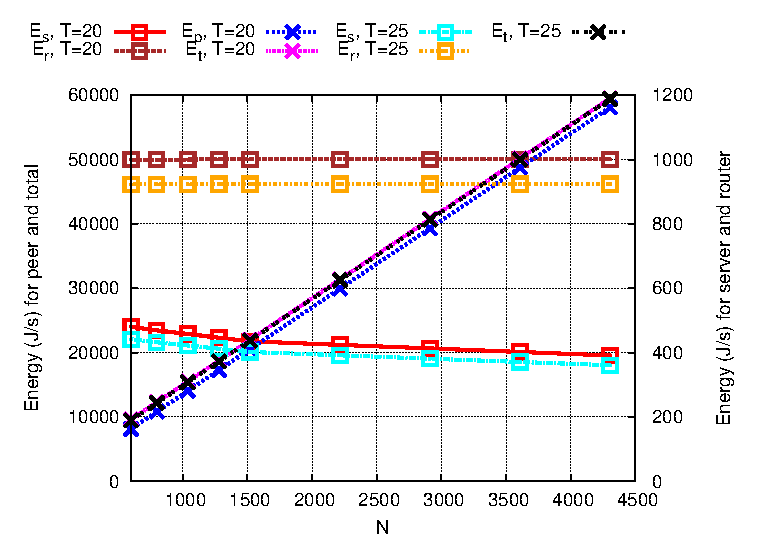
\includegraphics[scale=0.45]{graphs/lw-energy.eps}
	\caption{Power consumption for lower bound strategy.Left axes in log scale for peers and total power consumption. Right axes in linear scale for router and CDN server.}
	\label{fig:lw-energy}
\end{minipage}
\hfill
\centering
\begin{minipage}[b]{0.4\linewidth}
	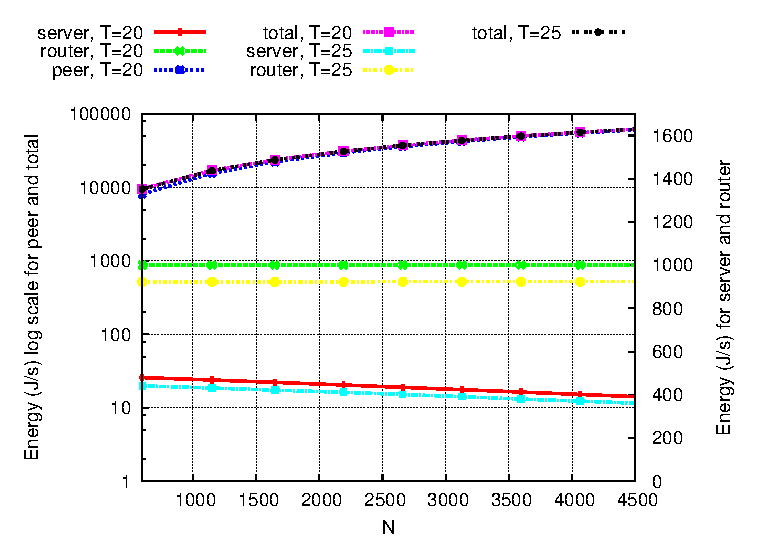
\includegraphics[scale=0.45]{graphs/req-energy.eps}
	\caption{Power consumption for request driven strategy.Left axes in log scale for peers and total power consumption. Right axes in linear scale for router and CDN server.}
	\label{fig:req-energy}
\end{minipage}
\hfill
\centering
\begin{minipage}[b]{0.4\linewidth}
	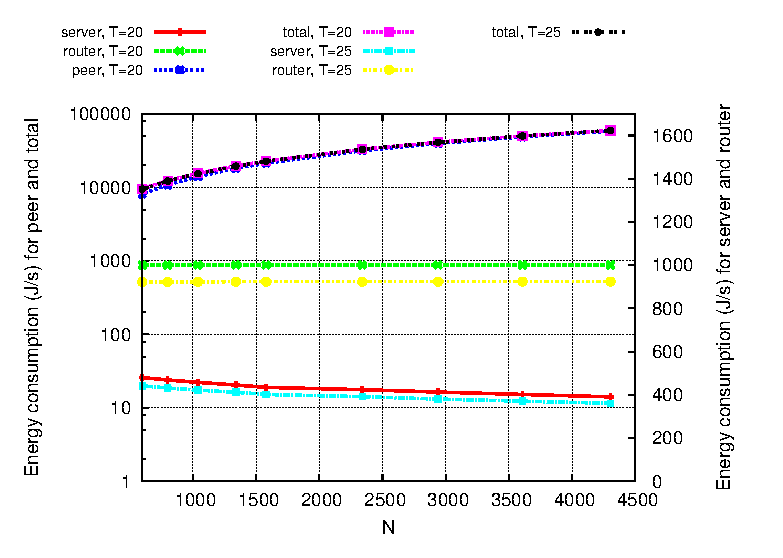
\includegraphics[scale=0.45]{graphs/wl-energy.eps}
	\caption{Power consumption for water-leveling strategy.Left axes in log scale for peers and total power consumption. Right axes in linear scale for router and CDN server.}
	\label{fig:wl-energy}
\end{minipage}
\hfill
\centering
\begin{minipage}[b]{0.4\linewidth}
	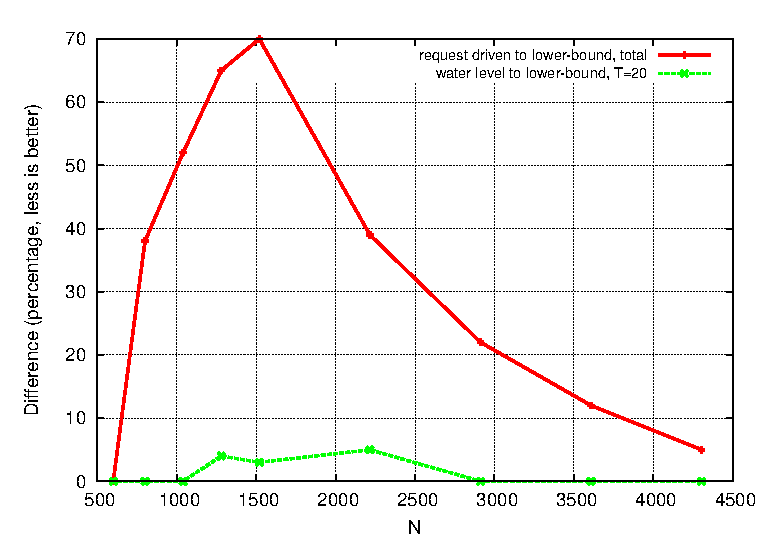
\includegraphics[scale=0.45]{graphs/diff-12.eps}
	\caption{Power consumption difference between request driven and water-leveling strategy to lower-bound strategy.}
	\label{fig:diff-12}
\end{minipage}
%\caption{main}
\label{fig:powereachstrategy}
\end{figure*}

\begin{figure*}[htp!]
\centering
\begin{minipage}[b]{0.3\linewidth}
	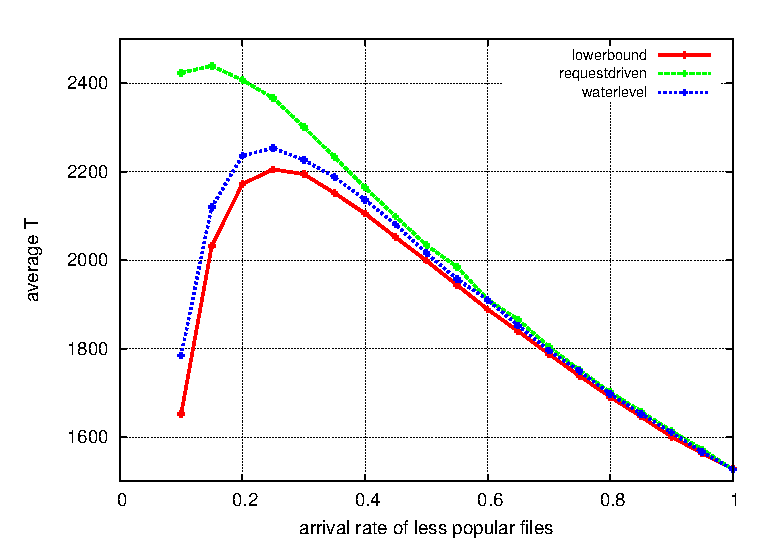
\includegraphics[scale=0.4]{graphs/pop.eps}
	\caption{Comparison of average downloading time under different server bandwidth allocation strategies when the peer arrival rate of less popular files varies.}
	\label{fig:popsimulation}
\end{minipage}
\hfill
\centering
\begin{minipage}[b]{0.3\linewidth}
	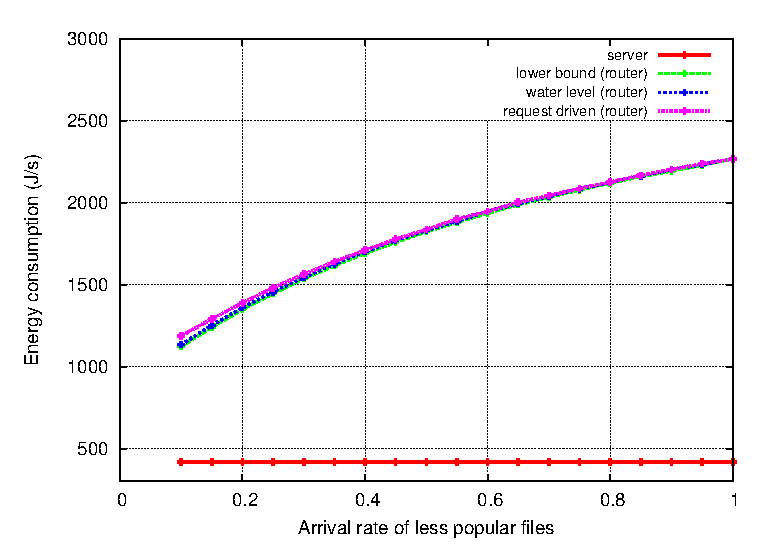
\includegraphics[scale=0.4]{graphs/componentconsumption.eps}
	\caption{Power consumption for server and router under different server bandwidth allocation strategies when the peer arrival rate of less popular files varies. Server bandwidth $S=50$MBps.}
	\label{fig:componentpop}
\end{minipage}
\hfill
\centering
\begin{minipage}[b]{0.3\linewidth}
	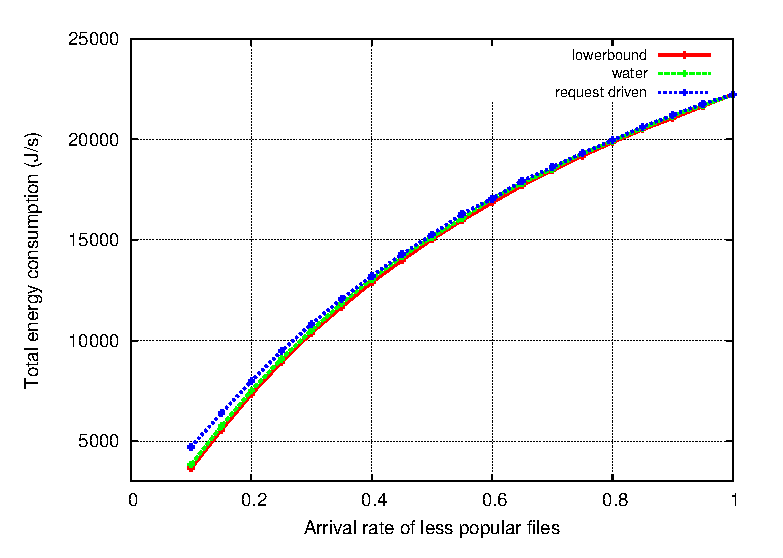
\includegraphics[scale=0.4]{graphs/totalconsumption.eps}
	\caption{Total power consumption under different server bandwidth allocation strategies when the peer arrival rate of less popular files varies. Server bandwidth $S=50$MBps.}
	\label{fig:totalpop}
\end{minipage}
\label{fig:popularity}
\end{figure*}


\subsection{Online Storage Case}\label{subsec:onlinestorage}

In peer-assisted online storage case, numerical simulation parameters that we used in this section same as \cite{Sun:2009:POS:1542245.1542249}.
Its parameters explanation and values are shown in sect.\ref{sec:parameters}.

Figures \ref{fig:lw-energy}, \ref{fig:req-energy}, and \ref{fig:wl-energy} show power consumption for every bandwidth strategy.
From fig.\ref{fig:lw-energy}, \ref{fig:req-energy}, and \ref{fig:wl-energy} we found that increasing number of peers can decrease CDN server power consumption because CDN server can reduce bandwidth or work due to increasing of peers that exchange blocks. 
We also found that router power consumption relatively flat. 
This is because compensation of server bandwidth reduction by increasing number of peers.  
Figure \ref{fig:diff-12} shows comparison energy consumption between request driven to lower bound strategy and water-leveling strategy to lower bound strategy.  
Compare to water-leveling strategy, request driven strategy required more energy than water-leveling strategy because request driven strategy equalizes the server bandwidth across all the peers.
Water-leveling strategy equalizes server bandwidth across all the files by taking file popularity into consideration thus minimize downloading time. 
This minimization result near to lower-bound strategy.  

%Request driven strategy totally consume around $12\%$ more energy compare to lower bound strategy fig.\ref{fig:diff2to1}, while water level strategy totally consume %around $2.3\%$ more energy compare to lower bound strategy fig.\ref{fig:diff3to1}.
%Compare to CDN architecture, peer-assisted CDN online storage can save total energy around $0.45\%$ if we add cooling overhead $T=20$ and around $0.8\%$ if we have %cooling overhead $T=25$ fig.\ref{fig:difftocdn} for above case. 
%Generally, increasing server bandwidth will decrease number of peers thus increasing CDN server energy consumption and decreasing router energy consumption. 
%Total energy consumption in every strategies depend on number peers.  

File popularity has strong correlation with downloading performance. 
We examine popularity by varying the peer arrival rate of less popular files.
Specifically we linearly increase file popularity from $0.1$ to $1$ and we choose server bandwidth $S=50$MBps which is quite constraint and similar to FS2You case.
As shown in fig.\ref{fig:popsimulation} when file popularity increases, downloading performance decrease first and increases again as files become more popular.
When file popularity is low there are fewer peers downloading the file and hence each of them can obtain relatively more sever bandwidth.
When file popularity is high peers can enjoy high file sharing effectiveness and hence high average downloading rates.
Semi popular files get the worst downloading performance in the system as difficulty in both file sharing among peers and requesting bandwidth from server.
In request driven strategy, we do not find such as U-shaped curve due to server bandwidth strategy that is equally divided across all peers and not affected by file popularity.

Figure \ref{fig:totalpop} shows total energy of system as function from file popularity.  
More popular files imply having more peers in the system thus increases total energy.  
While CDN server energy consumption is constant, router energy consumption is increases fig.\ref{fig:componentpop}. 



\section{Related Work} 

Content Distribution Networks with peer assist have been successfully deployed on the Internet, such as Akamai \cite{Huang:2008:UHC:1496046.1496064} and LiveSky \cite{Yin:2010:LEC:1823746.1823750}.  
The authors of \cite{Huang:2008:UHC:1496046.1496064} conclude from two real world traces that hybrid CDN-P2P can significantly reduce the cost of content distribution and can scale to cope with the exponential growth of Internet video content.  
Yin et al. \cite{Yin:2010:LEC:1823746.1823750} described LiveSkye as commercial operation of a peer-assisted CDN in China.  
LiveSky solved several challenges in the system design, such as dynamic resource scaling of P2P, low startup latency, ease of P2P integration with the existing CDN infrastructure, and network friendliness and upload fairness in the P2P operation.  
Measurement from LiveSky showed that LiveSky can save bandwidth around 40\% \cite{Yin:2010:LEC:1823746.1823750}.
The author in \cite{Huang:2007:IVP:1282427.1282396} and \cite{huang2007peer} proposed mechanisms to minimize CDN server bandwidth to make the content distribution cheap.
They designed different peer prefetching policies of video on demand system in surplus mode while ensuring user quality of experience.
A similar analysis has been done in \cite{xu2006analysis} for live video streaming system where the authors proposed different limited peer contribution policies to reduce CDN bandwidth requirement and eventually off the distribution process from CDN to P2P system. 
An ISP friendly rate allocation schemes for a hybrid CDN-P2P video on demand system in \cite{Wang:2008:IRA:1459359.1459397}. 
These technique try to minimize CDN server bandwidth while reducing ISP unfriendly traffic and maximizing peer prefetching.
Load on CDN server has been shown to be reduced using this approach while reducing cross ISP traffic.
Above studies were performed for video on demand or live video streaming.
While video is the most popular content, the systems can be also for other type contents.
Moreover while content based services are growing, energy consumption of a content distribution system has not been analyzed.

Related to CDN and energy usage, in a seminal work \cite{qureshi2009cutting}, the authors show that if costs are based on electricity usage and if the power prices vary in real-time, global load balancing decision can be made such that users are routed to locations with the cheapest power without significantly impacting user performance or bandwidth cost.  
In \cite{Palasamudram:2012:UBR:2391229.2391240}, the author proposed utilizing batteries for CDN for reducing total supplied power and total power costs.
The authors in \cite{Palasamudram:2012:UBR:2391229.2391240} also proposed battery provisioning algorithms based on workload of CDN server. 
The result shows that batteries can provide up to 14\% power savings.

The idea that utilize ISP controlled home gateway to provide computing and storage services and adopts managed peer-to-peer model is presented in \cite{valancius2009greening}. 
Valancius et al. \cite{valancius2009greening} show that distributing computing platform in NaDa (Nano Data Center) save at least 20-30\% energy compare to traditional data centers.
The saving in NaDa comes from underutilizing home gateway, avoidance of cooling costs, and the reduction of network energy consumption as a result of demand and service co-localization.

The comparison between CDN architecture and peer-to-peer architecture are discussed in \cite{baliga2007energy} and \cite{feldmann2010energy}.
Both authors in \cite{baliga2007energy} and \cite{feldmann2010energy} agree that CDN architecture is more energy saving compare to peer-to-peer architecture. 
Another interesting study of energy efficient in content delivery architectures is presented by Guan et al. \cite{5963557}.
by Guan et al. \cite{5963557} comparing energy efficient of CDN architecture and CCN architecture.
The authors in \cite{5963557} conclude that CCN is more energy efficient in delivering popular content while the approach with optical bypass is more energy efficient in delivering infrequent accessed content.

To the best of our knowledge, the study of energy in that considering peer-to-peer in CDN architecture is presented in \cite{6524219}.
Mandal et al. \cite{6524219} mentioned that hybrid CDN-P2P systems can reduce a significant amount energy in the optical core network around 20-40\% less energy.  
The authors only considered energy consumption of hardware especially optical devices and does not include overhead inside data center, CDN server energy consumption, and consumed power by peers.
Our work is quite different, we take number of peers and add overhead of data center which is power of cooling cause by temperature of hardware for different purpose: live streaming and online storage.

\section{Conclusion and Future Work}\label{conclusion}

In this paper, we have introduced the comparison of energy consumption between the peer-assisted CDN architecture and CDN architecture for live streaming and video on demand service.
Integrating peer to peer capability to assist the existing CDN has a potential to save energy consumption.
In this study, we show that event without explicitly considering energy consumption while assigning content, the peer assisted CDN can save energy consumption.
Although the energy savings depend on number of request (number of clients), number of router and its configuration, for total system energy saving is around $0.5$ to $1.2$.
If we break per component in live streaming case, the CDN server is the part that can be pushed to save energy up to $11\%$ and can be more if new generation of power proportional server is used \cite{Krioukov:2011:NDI:1925861.1925878}.
Unfortunately, in peer-assisted online storage, we do not see such energy saving.  
In peer-assisted storage, all of strategies that we discussed before focus how to efficiently allocated bandwidth from CDN server for every peers.
CDN server is fully used to serve peers, thus we do not see energy saving in CDN server.
We agree with \cite{4509688}, Router component in the other side is quite difficult to optimize for energy saving, because different chassis size, different network interface type slot, and different configuration can lead to different energy consumption.
Different COP values, in our case $T=20$ and $T=25$, only give $7\%$ difference power consumption.
Obviously, with $T=25$ overhead is minimal compare to $T=20$.
Once again, It is not our aim to advocate air cooling supply temperature value over another since there is reliability issue related to hardware.  
We only show that increasing temperature can minimize overhead.
Several areas that we have been identified for future work are: more correlation analysis of time period to peer energy usage pattern in live streaming, continued characterization of different peer energy usage based on flash memory storage, and comparing energy model with different file popularity models.


\section*{Acknowledgements}
We thank A,B,C, and D

\bibliographystyle{IEEEtran}% bib style
\bibliography{journal}% your bib database



%\begin{biography}
%
%\profile{Mohamad Dikshie Fauzie}{was born in 1976.\
%He received a bachelors degree and a master's degree from Institute of Technology Bandung, Indonesia.\
%He is currently a Ph.D candidate at Keio University's Shonan Fujisawa Campus.}
%
%\profile{Achmad Husni Thamrin}{is Assistant Professor at Keio University.\ 
%He is a graduate of Keio University, Graduate School of Media and Governance (Ph.D 2005, MMG, 2002).\
%His research interests include multicast, Internet over broadcast media, and peer-to-peer networks.} 
%
%\profile{Jun Murai}{was born in March 1955 in Tokyo.\
%Graduated Keio University in 1979, Department of Mathematics, Faculty of Science and Technology.\
%He received his M.S. for Computer Science from Keio University in 1981,
%and received his Ph.D. in Computer Science, Keio University in 1987.\ 
%He specializes in computer science, computer network, and computer 
%communication. He is currently Dean of the Faculty of Environment and Information Studies, Keio University since October 2009.\
%Former Vice-President of Keio University from May 2005 to May 2009.\ 
%He was an Executive Director of the Keio Research Institute at SFC, Keio University from 1999 to 2005.}
%
%\end{biography}

\end{document}
